\section{Results}

% \begin{figure*}
%  \subfigure[EHP vs. Light]{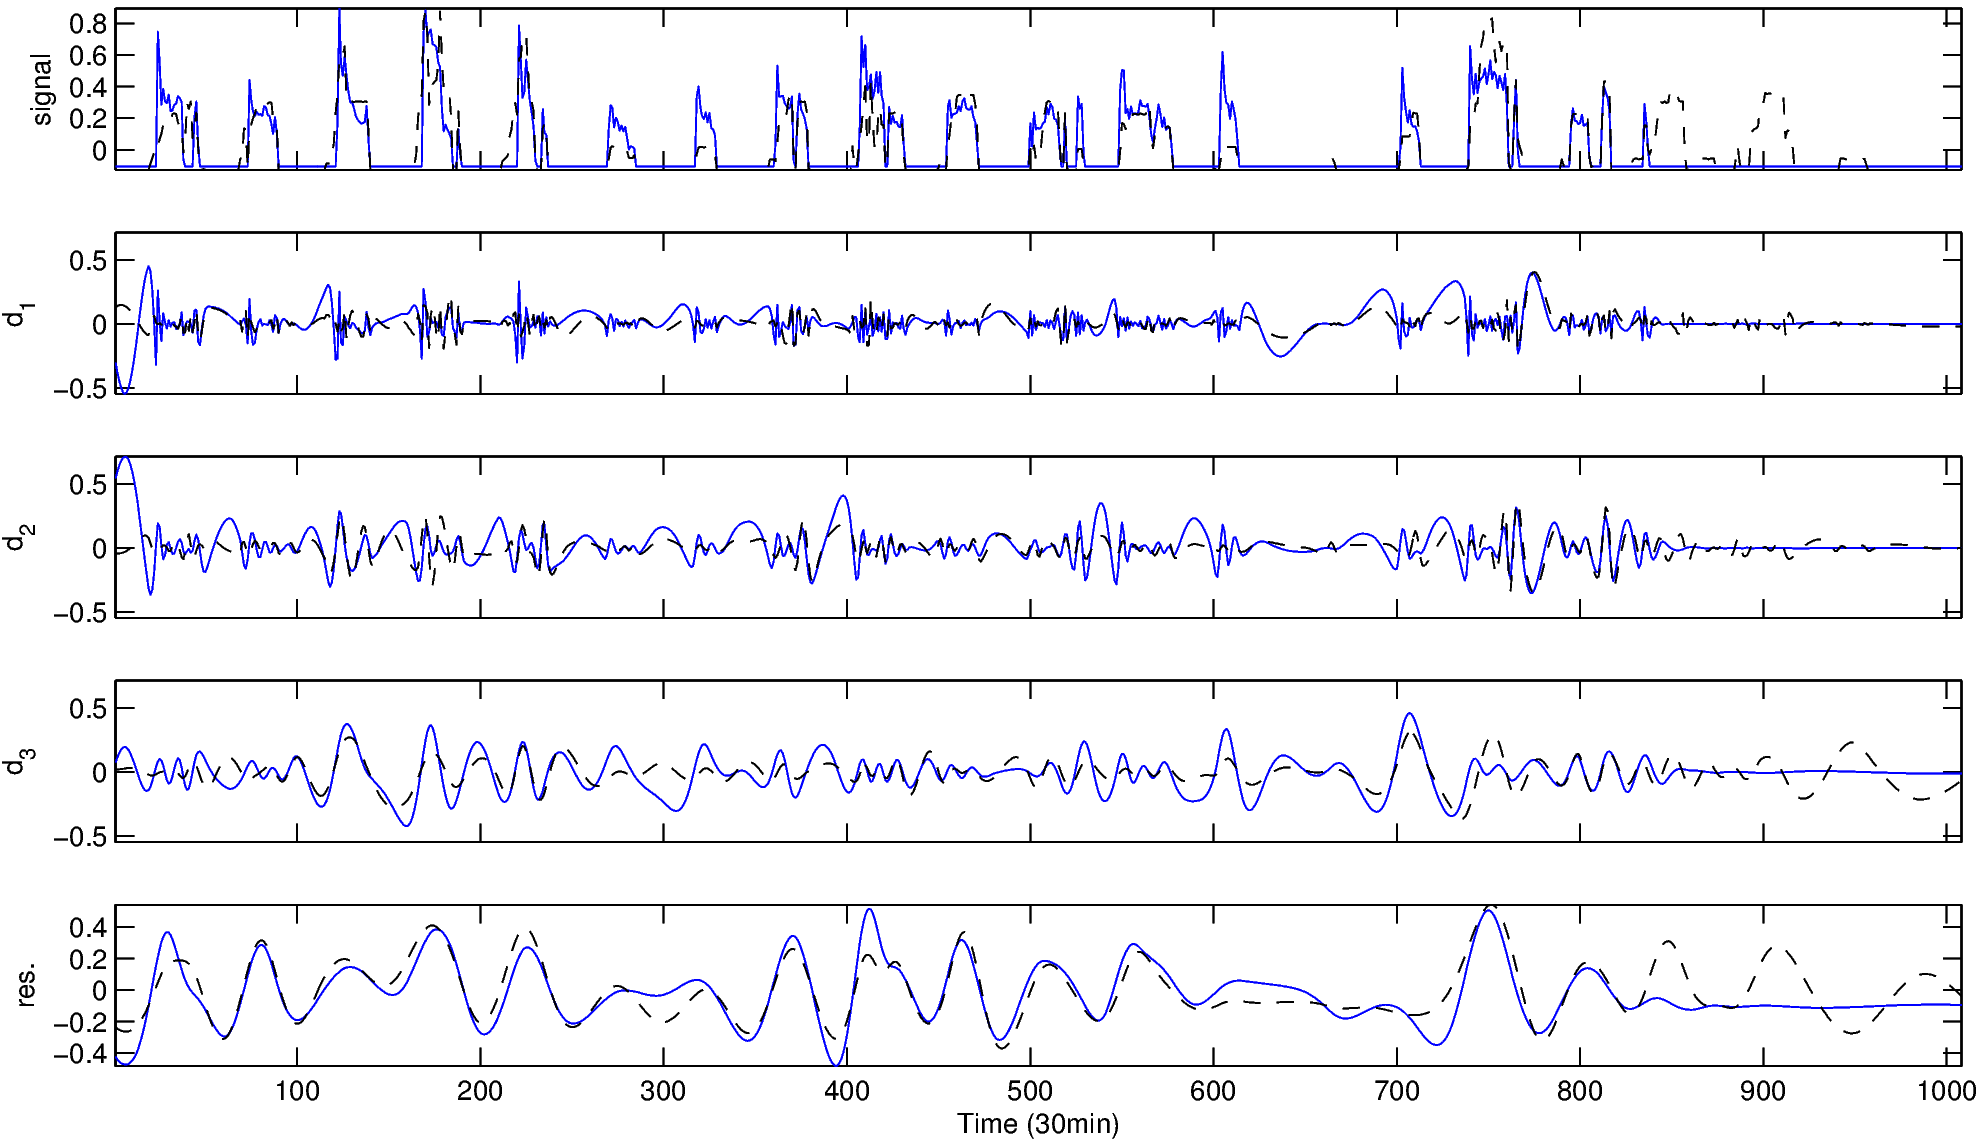
\includegraphics[width=\textwidth]{img/emd_25_26}}
%  \subfigure[EHP vs. GHP]{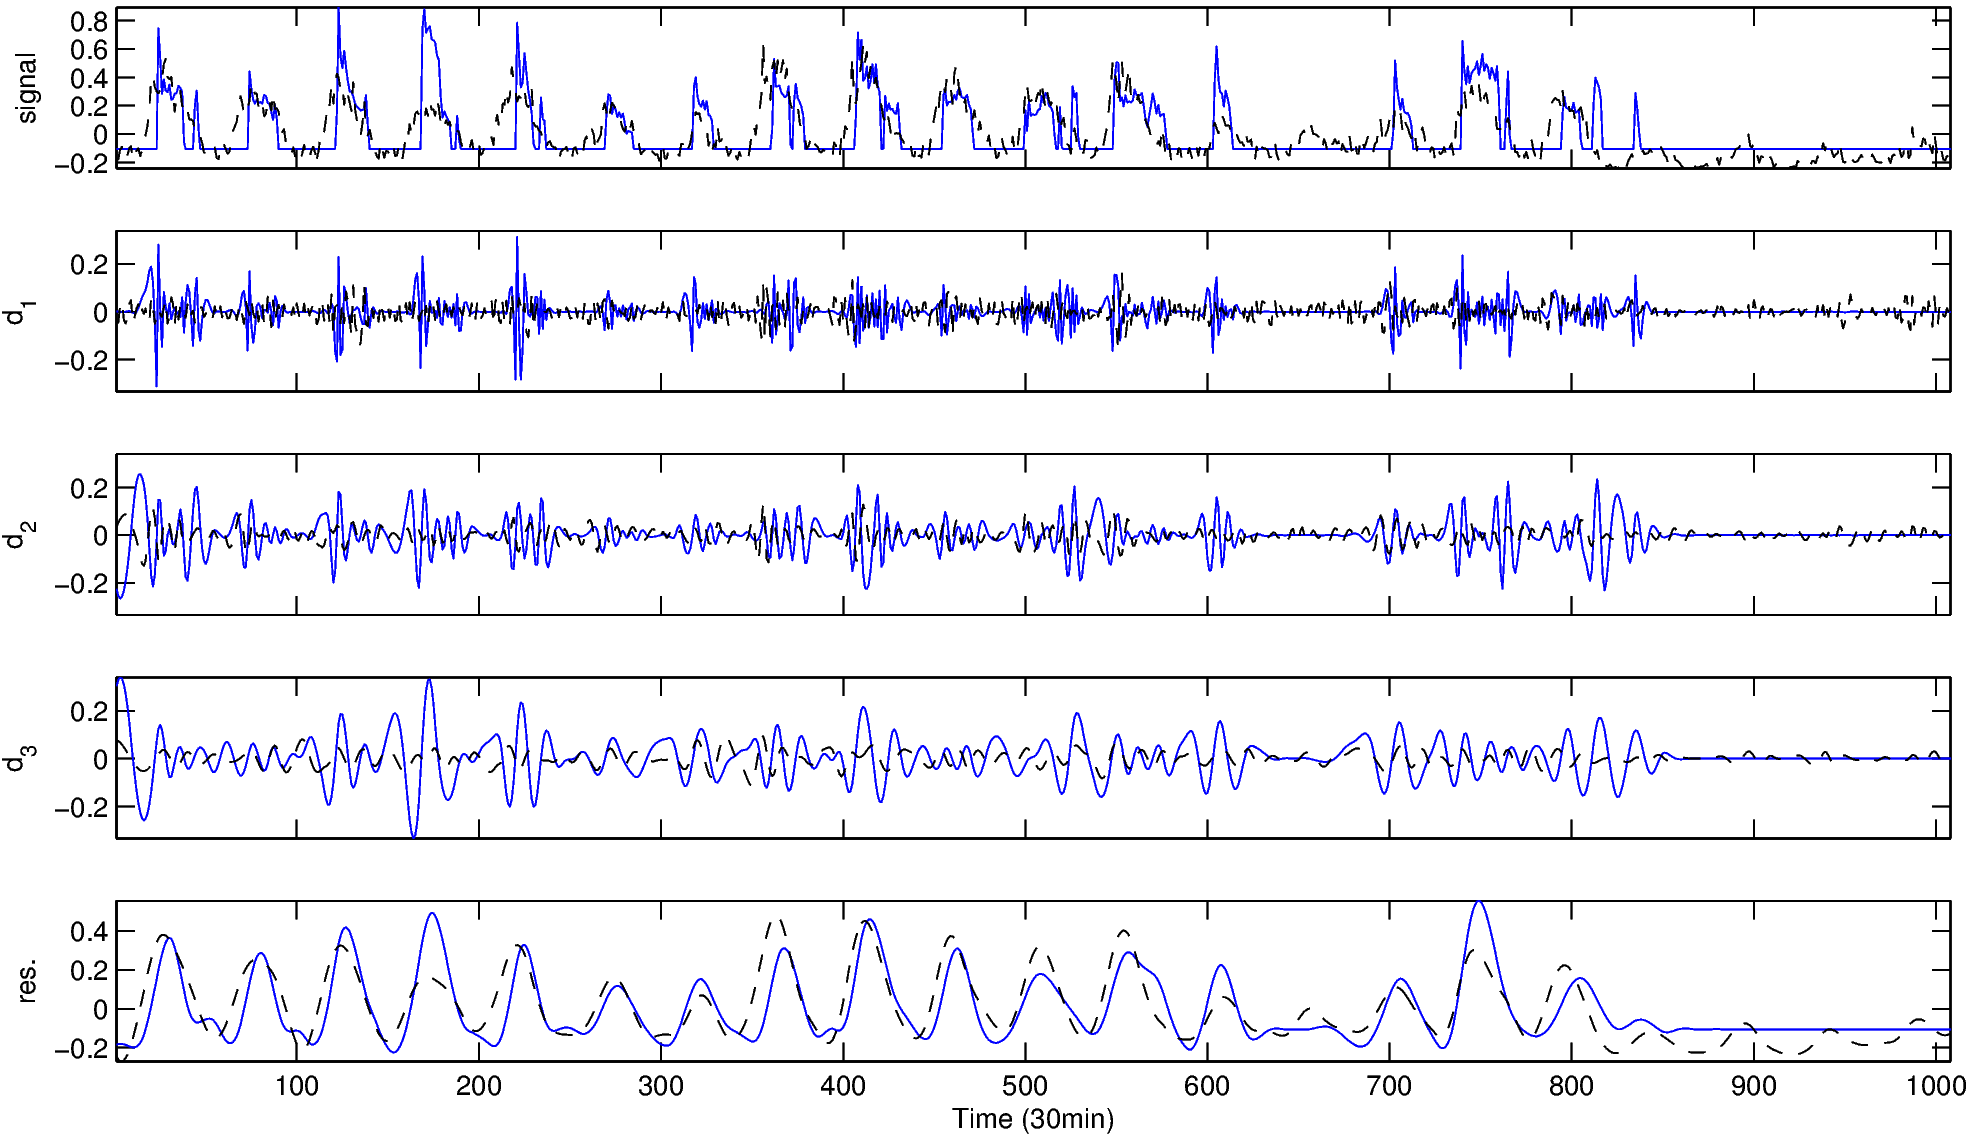
\includegraphics[width=\textwidth]{img/emd_25_41}}
%  \caption{Empirical Mode Decomposition}
%  \label{fig:emd}
% \end{figure*}

\begin{figure*}[tb]
\begin{center}
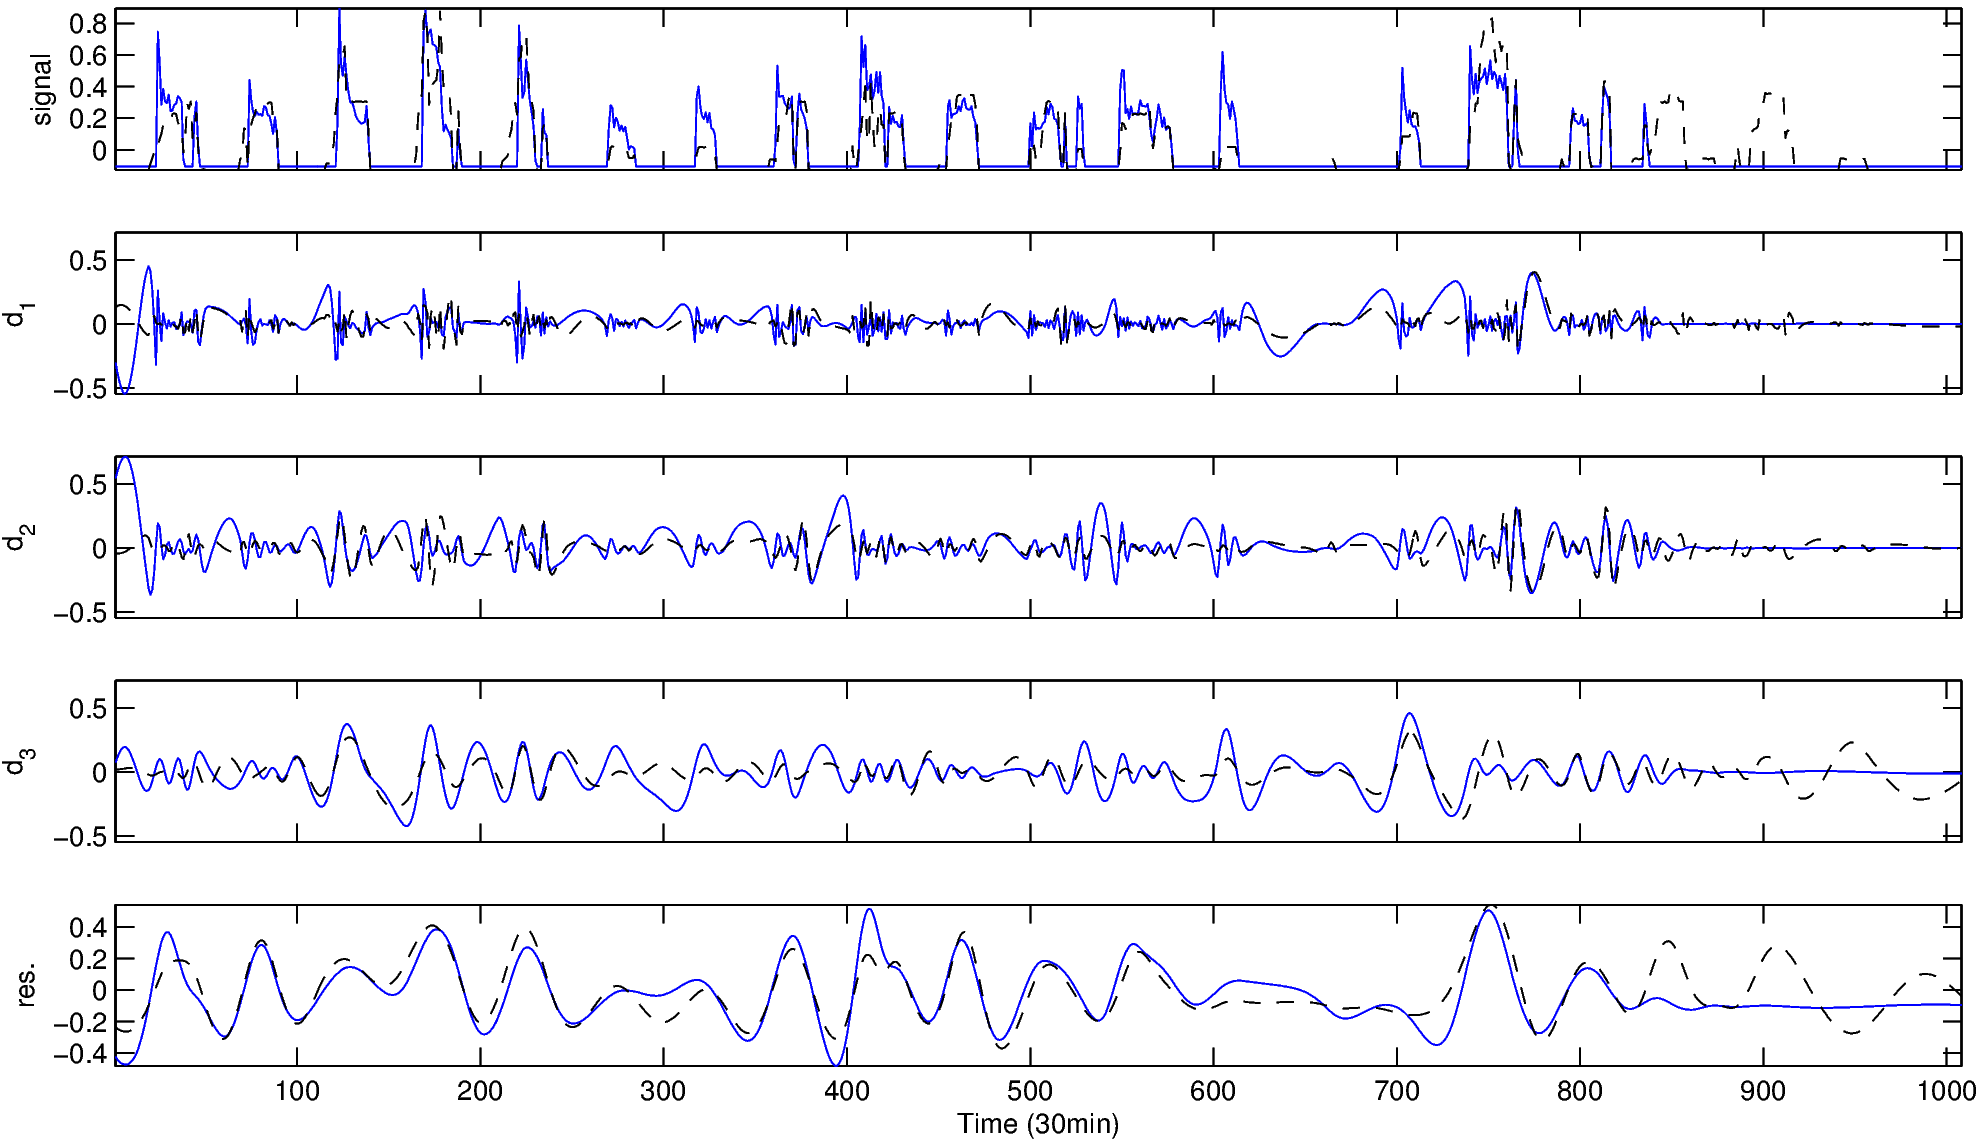
\includegraphics[width=\textwidth]{img/emd_25_26}
\caption{}
\label{fig:emd}
\end{center}
\end{figure*}

This section emphasizes the advantages of EMD to effectively uncover correlated sensor traces.
First, we demonstrate the benefit of EMD with a simple example, the three sensors presented in Section \ref{problem}.
Second, we validate the proposed methodology using a large dataset (674 sensors) and highlight the ability of EMD to uncover the spatial correlations of the sensors.

\begin{table*}
\begin{center}
\begin{tabular}{|l|l|l|l|l|l|}
\hline
× & Raw trace & 1st IMF & 2nd IMF & 3rd IMF & Residual\\ \hline
EHP, Light & 0.7715 & 0.43909 & 0.49344 & 0.63469 & 0.82132 \\ \hline
EHP, GHP & 0.6370 & 0.0060274 & 0.063546 & 0.16764 & 0.79378 \\ \hline
\end{tabular}
\caption{Correlation coefficients of the analyzed trace and their IMFs uncovered by EMD}
\label{tab:corr}
\end{center}
\end{table*}
\subsection{Simple Scenario}

\begin{figure*}[tb]
\begin{center}
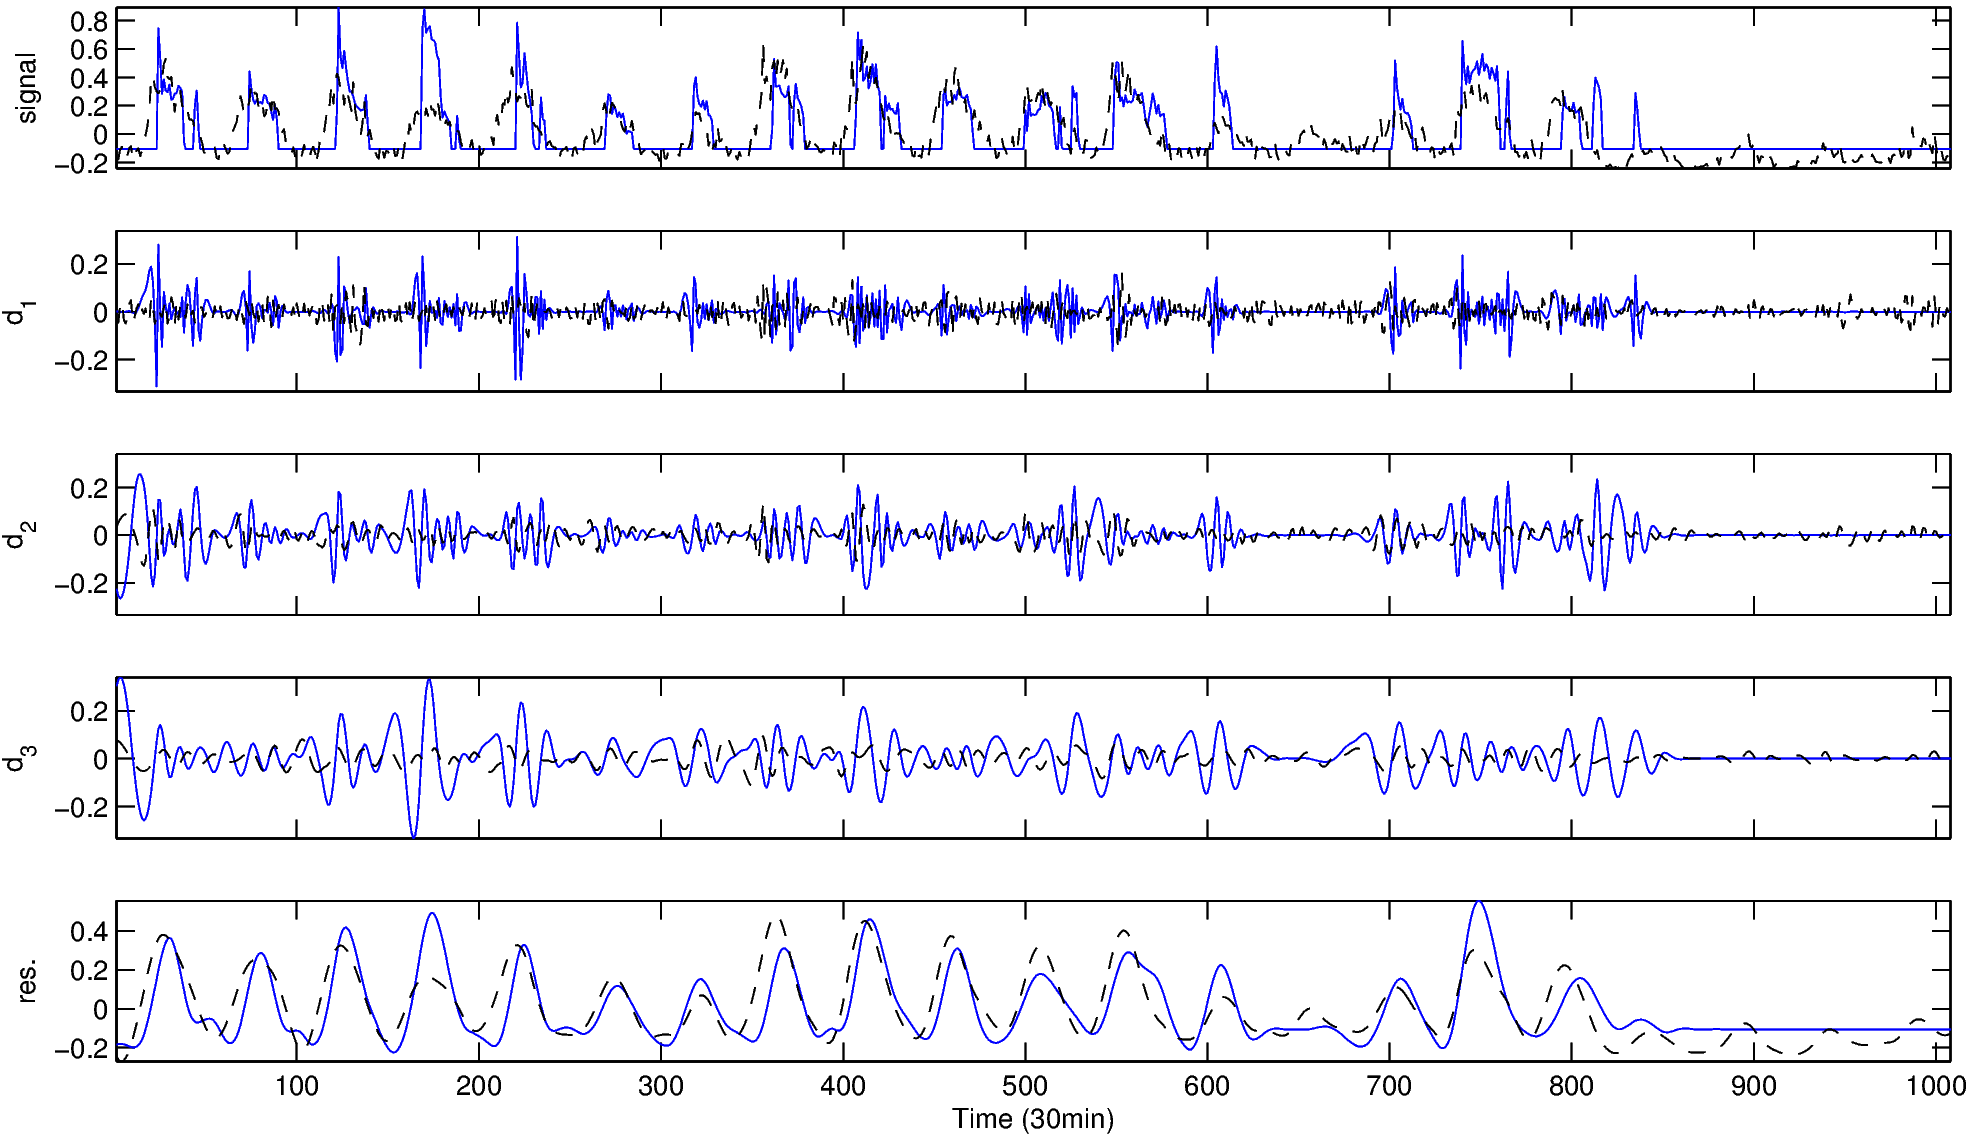
\includegraphics[width=\textwidth]{img/emd_25_41}
\caption{}
\label{fig:emd2}
\end{center}
\end{figure*}

Lets consider the simple example of Section \ref{problem} where we would like to know if the EHP trace is correlated with the two other traces; a light trace and a GHP trace.
Using the raw traces, the correlation coefficients $0.7715$ and $0.6370$ corresponding respectively to the light and GHP trace suggest that both traces are correlated to the EHP trace (Table \ref{tab:corr}).
As stated in previous section this result is certainly biased by the strong daily pattern shared by these three traces.

We emphasize that extracting the daily pattern of the data using EMD permits a more detailed analysis of these traces.
Figure \ref{fig:emd} depicts the EMD decomposition of the three traces.
Notice that the EMD process has been voluntary stopped once the daily pattern has been uncovered.
Thereby, for each trace EMD has retrieved three IMFs that highlight the high frequency domain of the traces.

The correlation coefficients for the EHP and light IMFs --- i.e. $0.43909$, $0.49344$ and $0.63469$ corresponding respectively to the IMF1, IMF2 and IMF3 --- emphasize the positive correlation of the two traces in the high frequency domain.
However, the correlation coefficients for the EHP and GHP IMFs show that the two traces are independent in the high frequency domain.
Therefore, EMD permits to effectively identify that the light trace is related to the EHP whereas the GHP one is not.

\begin{figure}[tbh!]
\centering
 \subfigure[Raw traces correlation coefficients]{\label{fig:histo1}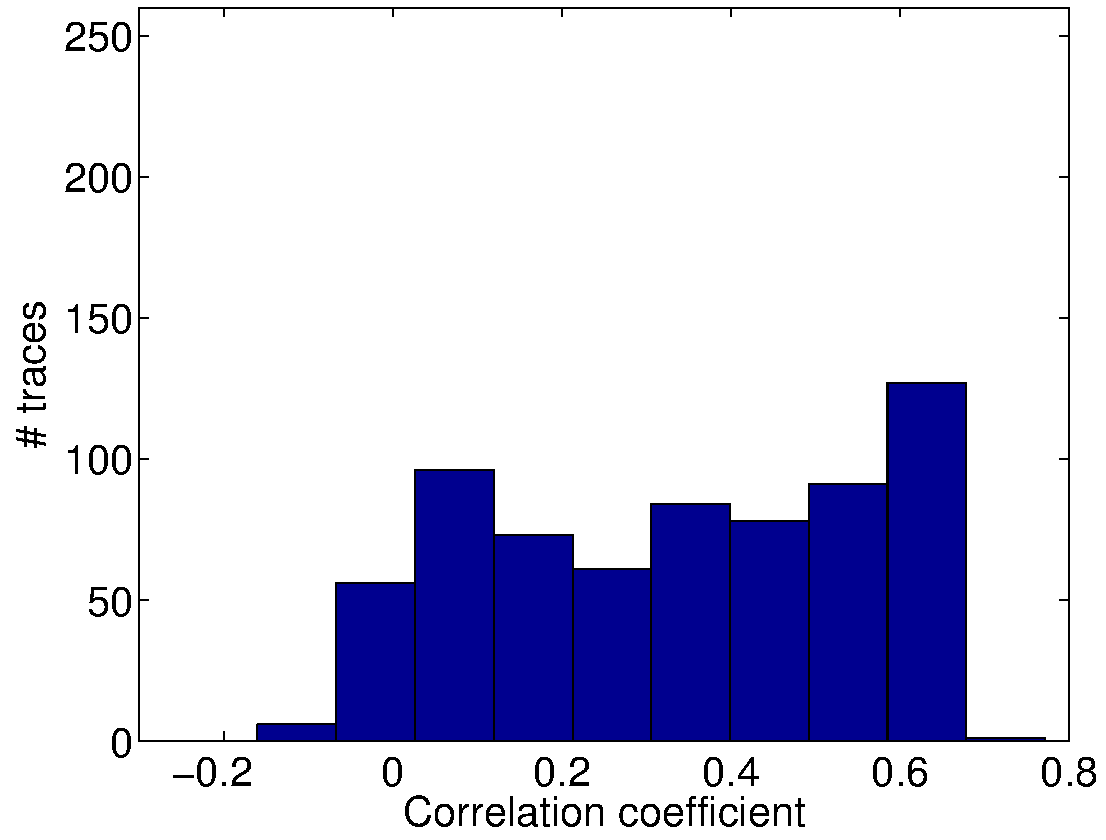
\includegraphics[width=.45\textwidth]{img/allFloors_week1_week4_corr_abs-eps-converted-to}}
 \subfigure[Average IMFs correlation coefficients]{\label{fig:histo2}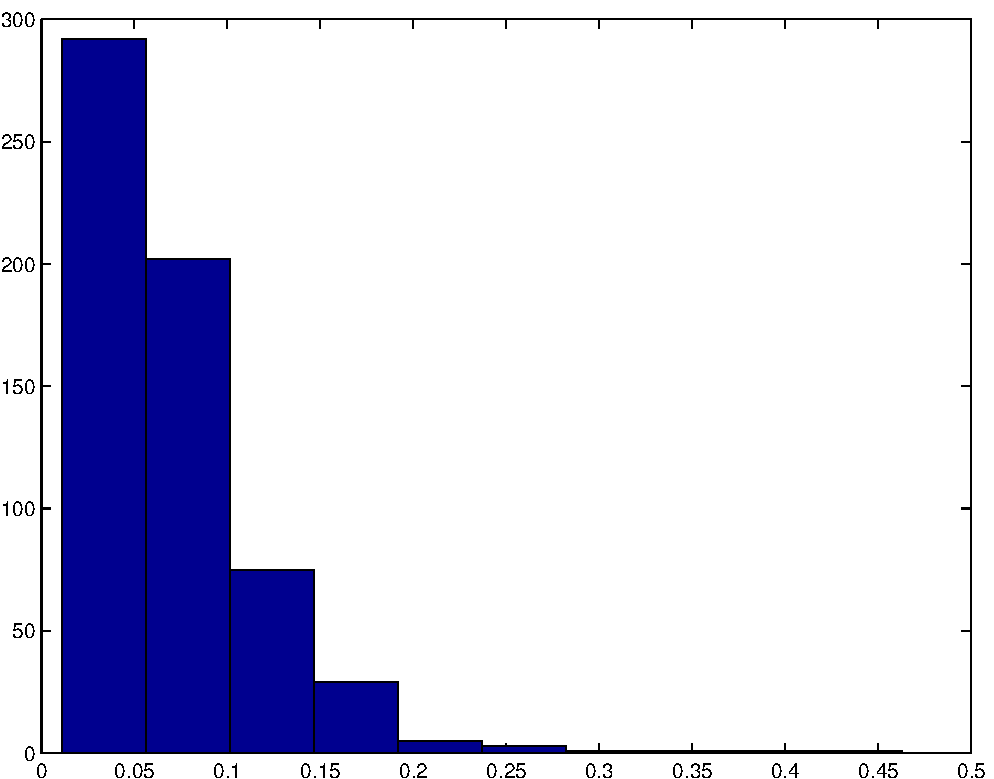
\includegraphics[width=.45\textwidth]{img/allFloors_week1_week4_emd_abs-eps-converted-to}}
 \caption{Distribution of the correlation coefficients of the raw traces and corresponding IMFs using 3 weeks of data from 674 sensors deployed on 12 Floors.}
\label{fig:histo}
\end{figure}

\subsection{Validation}


In order to validate the effectiveness of the proposed approach to identify correlated traces, we analyze three week traces from the 674 sensors deployed in the building.
For each trace $S$ we compute two scores: (1) the correlation coefficient for $S$ and the EHP trace, (2) the average value of the two traces IMFs correlation coefficients.

Figure \ref{fig:histo1} shows the distribution of the traces correlation coefficients.
Regarding this figure a large fraction of the dataset seems to be correlated with the EHP trace.
Indeed half of the analyzed traces provide a correlation coefficient higher than $0.36$.
Although the highest score (i.e. $0.7715$) corresponds to the light trace that is from the same room as the EHP trace thus actually related to it, all the traces that achieve a score higher than $0.6$  correspond to 118 heat pumps that are located at different floors and are independent from the analyzed EHP trace.
Moreover, the distribution of the traces is almost uniform, thus, discriminating correlated traces is a laborious task.

Figure \ref{fig:histo2} shows the distribution of the average correlation coefficients for the IMFs of each trace and the analyzed EHP one.
The number of traces correlated in the high frequency domain is significantly small compared to previous results. 
Only 10 traces perform a score higher than $0.25$ and their distribution allow us to easily rank traces in term of correlation.

Interestingly the IMFs correlation coefficients reveal the spatial correlation of the sensors.
Figure \ref{fig:map} is the map floor where the EHP trace is measured.
Specifically, the EHP reports heating activity in the room $C2$.
Regarding the results from the IMFs correlation coefficients, the trace performing the highest score (i.e. $0.522$) is the trace corresponding to the lighting system of the same room.
The two highest scores for this floor (i.e. $0.316$ and $0.279$) are the light and EHP traces from next door, room $C1$.
Lower values correspond to sensors measuring activities in other rooms that have no specific relations with the analyzed trace.
% in the simple scenario the GHP is located in the room A5.

\begin{figure}
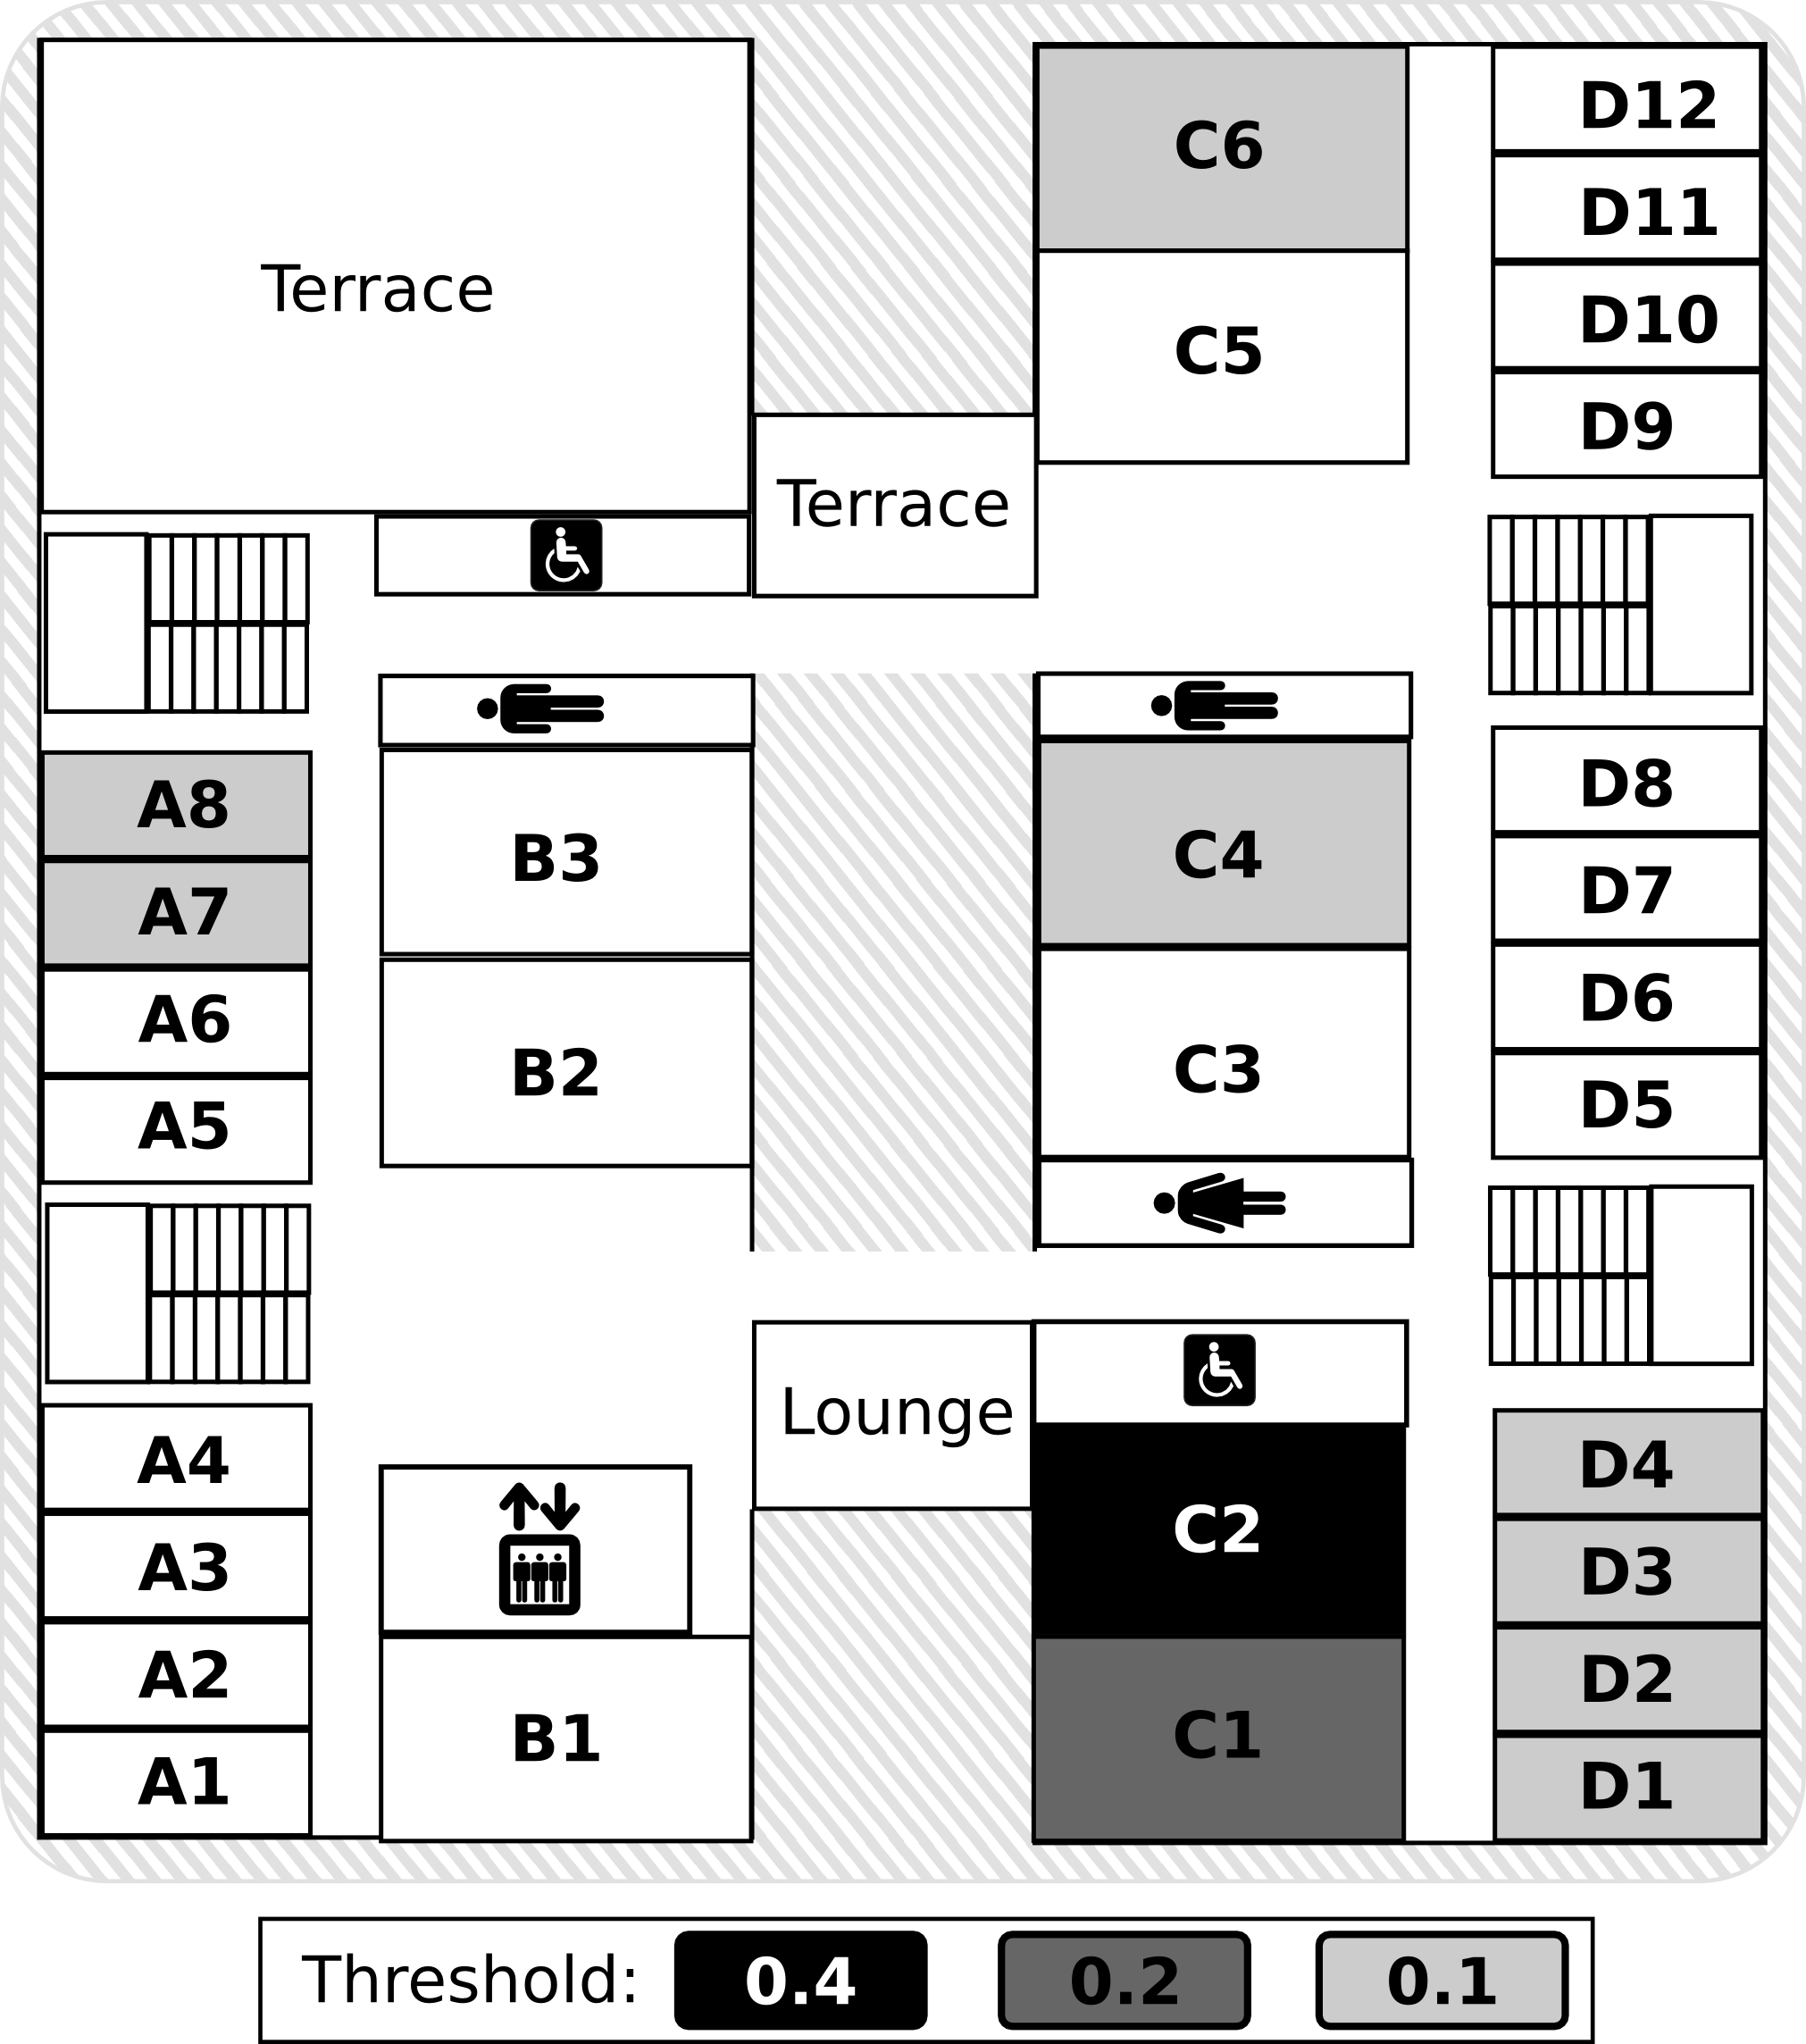
\includegraphics[width=.5\textwidth]{img/floorMap.png}
\caption{}
\label{fig:map}
\end{figure}
